\section{System Design and Implementation}\label{sec:system}
Fig.~\ref{fig:arch} shows the architecture. A React~19/TypeScript client talks to an
asynchronous FastAPI backend over REST and Server-Sent Events (SSE); uploads are streamed to
local disk or S3-compatible object storage (Cloudflare R2, S3, MinIO) with SHA-256 integrity
hashes; relational data (users, events, jobs, transcripts, content, embeddings, audit log) is
kept in PostgreSQL or SQLite. Jobs run as in-process background tasks or Celery workers.
All model calls go to Google Cloud Vertex AI using Application Default Credentials, so no API
key is stored in the application.

\begin{figure*}[t]
  \centering
  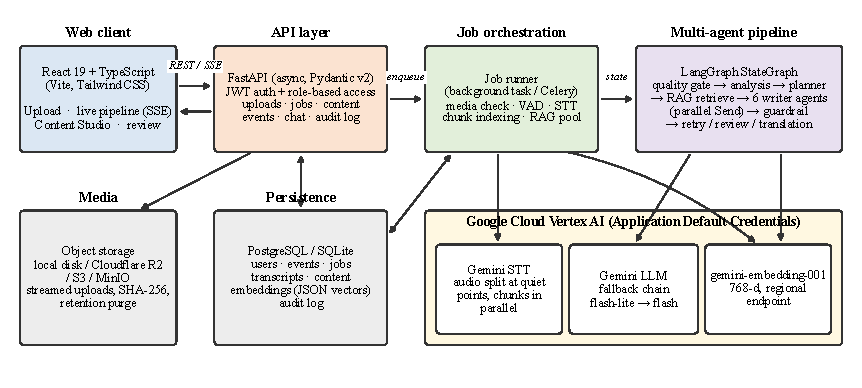
\includegraphics[width=\textwidth]{fig_architecture}
  \caption{EventAI architecture. Arrows show request and data flow; all model calls use
  Vertex AI with Application Default Credentials.}
  \label{fig:arch}
\end{figure*}

\subsection{Ingestion and speech-to-text}
An organiser uploads audio, video or a text transcript after confirming that participants
consented to processing. The job runner validates the file (extension whitelist, size and
duration limits, optional ClamAV scan), measures duration, sample rate and silence ratio, and
applies a voice-activity pre-check that rejects recordings with no detectable speech.
Transcription uses Gemini on Vertex AI. Because Vertex accepts at most about 20\,MB of inline
audio per request, the recording is resampled to 16\,kHz mono and split into windows of
300\,s; each window end is moved to the quietest 250\,ms frame within the preceding 10\,s so
that boundaries fall between words. Chunks are transcribed concurrently (four at a time)
and concatenated. If the engine fails, the runner tries every other configured engine
(Gemini API, VideoDB) in turn, skipping engines whose credentials were rejected at start-up.

\subsection{Multi-agent pipeline}
The pipeline is a LangGraph \texttt{StateGraph} (Fig.~\ref{fig:pipeline}). A quality gate
routes low-confidence transcripts to \texttt{needs\_reupload}. An \emph{analysis} node
extracts topics, highlights, speaker characteristics, tone and an editorial brief (angle,
key messages, audience, verbatim quotes) in one structured JSON call; a \emph{planner} node
reuses this brief. After selective RAG (Section~\ref{sec:rag}), the LangGraph \texttt{Send}
API fans out to the six requested writer agents in parallel: executive summary, blog
article, LinkedIn post, newsletter, Instagram caption and event flyer. Each agent is defined
by a Markdown \emph{skill} file (persona, structure, do/don't rules, an example) plus the
author's profile (name, organisation, tone, sign-off). Writers see the first 12{,}000
characters of the transcript, the brief and the retrieved excerpts, and must return JSON.

\begin{figure*}[t]
  \centering
  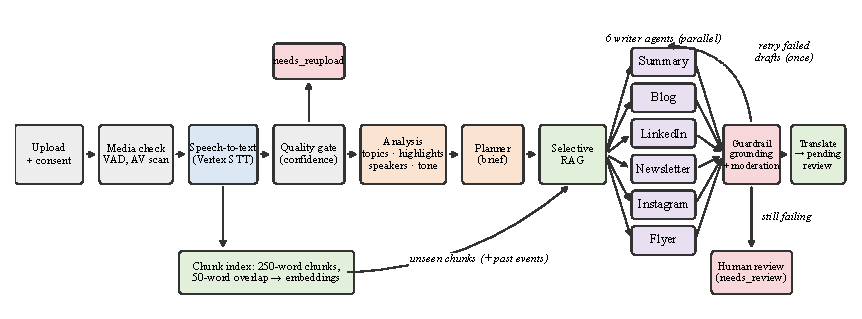
\includegraphics[width=\textwidth]{fig_pipeline}
  \caption{LangGraph pipeline. Only drafts that fail the guardrail are regenerated, once;
  drafts still failing are routed to human review, the rest are translated.}
  \label{fig:pipeline}
\end{figure*}

\subsection{Guardrail and human review}
A single batched LLM call checks all drafts at once for \emph{grounding} (claims not
supported by the transcript) and \emph{moderation}. The guardrail receives the full
transcript and the author profile, so that user-supplied sign-offs are not flagged as
invented. Drafts that fail are regenerated once---only the failing types, skipping the
planner---and drafts that still fail are routed to human review; otherwise the job proceeds
to translation, in which each target language is one batched call for all drafts. Every
draft then waits for approval in the Content Studio, where it can be edited, approved,
copied or exported; nothing is marked ready to publish automatically.

\subsection{Selective retrieval-augmented generation}\label{sec:rag}
Transcripts are split into overlapping 250-word chunks (50-word overlap) and embedded with
\texttt{gemini-embedding-001} (768 dimensions); vectors are stored in a JSON column, so no
database extension is needed. Retrieval is \emph{selective}: it runs only when the
transcript exceeds what the writers see directly ($>$2{,}000 words) or when the organiser
enables organisation memory. The candidate pool excludes chunks already inside the writers'
12{,}000-character excerpt and, with organisation memory, adds chunks from the organiser's
earlier events. A \texttt{rag\_retrieve} graph node builds the query from the editorial
brief (angle, key messages, topics and highlights) and passes the top $k{=}6$ chunks, by
cosine similarity, to every writer, labelled as later parts of this session or as earlier
events that must not be presented as said in this session. If the embedding service is
unavailable, a hashed bag-of-words representation is used instead.

\subsection{Resilience}
Every model call has a timeout (60\,s) and an immediate retry for transient errors. The
Vertex provider always starts with the configured model and walks a fallback chain
(\texttt{gemini-3.1-flash-lite}, then \texttt{gemini-3.6-flash}) when a model returns an
error, a permanent ``not found'' or an empty response. Each model has its own circuit
breaker: after three consecutive failed calls the model is skipped for 60\,s and then tried
again; a model that answered ``not found'' is skipped for the rest of the process. Every
model reply is coerced to a JSON object. If every model fails, an offline template generator
keeps the job running, but the job is flagged as degraded and routed to human review.
Provider credentials are checked at start-up, and speech-to-text falls back through every
configured engine whose credentials were accepted. This is the version after the fixes of
Section~\ref{sec:discussion}; the differences to the version used in most live runs are
listed there.

\subsection{Implementation}
The backend is Python 3.11 (FastAPI 0.115, LangGraph 0.3.31, SQLAlchemy 2.0, google-genai);
the frontend is React~19, TypeScript and Vite with Tailwind CSS. The system is configured by
environment variables (provider, models, RAG threshold, $k$, embedding region) and ships with
Docker Compose files.
